\PassOptionsToPackage{table}{xcolor}
\documentclass[sigconf]{acmart} %% CCS: DO NOT REMOVE

\AtBeginDocument{%
  \providecommand\BibTeX{{%
    Bib\TeX}}}

\setcopyright{acmlicensed} %% CCS: DO NOT REMOVE
\copyrightyear{2018} %% CCS: DO NOT REMOVE
\acmYear{2018} %% CCS: DO NOT REMOVE
\acmDOI{XXXXXXX.XXXXXXX} %% CCS: DO NOT REMOVE
\acmConference[Conference acronym 'XX]{Make sure to enter the correct
  conference title from your rights confirmation email}{June 03--05,
  2018}{Woodstock, NY} %% CCS: DO NOT REMOVE
\acmISBN{978-1-4503-XXXX-X/2018/06} %% CCS: DO NOT REMOVE
\settopmatter{printacmref=false}
\renewcommand\footnotetextcopyrightpermission[1]{}

\usepackage{amsmath}
\usepackage{algorithm}
\usepackage{algorithmic}
\usepackage{graphicx}
\usepackage{textcomp}
\usepackage{booktabs}
\usepackage{multirow}
\usepackage{mathrsfs}
\usepackage{pifont}
\usepackage{tcolorbox}
\usepackage{tikz}
\usepackage{enumitem}
\usepackage{tabularx}
\usepackage{balance}
\usepackage{placeins}
\usepackage{stfloats}

\usetikzlibrary{shapes,arrows,positioning,calc,fit,backgrounds}

\usepackage{cryptodef}
\setlength{\emergencystretch}{2em}
\flushbottom

% Unified visual style for algorithm/construction boxes and tables.
\tcbset{
  algobox/.style={
    colback=white,
    colframe=black,
    colbacktitle=gray!10,
    coltitle=black,
    fonttitle=\scriptsize\bfseries,
    boxrule=0.7pt,
    arc=0mm,
    toptitle=0.45mm,
    bottomtitle=0.45mm,
    titlerule=0.4pt,
    left=0.9mm, right=0.9mm, top=0.45mm, bottom=0.55mm,
    boxsep=0pt,
    before skip=2pt,
    after skip=2pt,
    before upper={%
      \setlength{\abovedisplayskip}{1.2pt plus 0.5pt minus 0.5pt}%
      \setlength{\belowdisplayskip}{1.2pt plus 0.5pt minus 0.5pt}%
      \setlength{\abovedisplayshortskip}{0.8pt plus 0.5pt minus 0.5pt}%
      \setlength{\belowdisplayshortskip}{0.8pt plus 0.5pt minus 0.5pt}%
      \setlength{\jot}{0.5pt}%
    }
  }
}
\newcommand{\TableStyle}{\setlength{\tabcolsep}{3pt}\renewcommand{\arraystretch}{1.06}}
\newcommand{\TableStyleTight}{\setlength{\tabcolsep}{2.6pt}\renewcommand{\arraystretch}{1.03}}

\newif\ifsubmission
\ifdefined\submissionbuild
  \submissiontrue
\else
  \submissionfalse
\fi

\setlength{\textfloatsep}{4pt plus 1pt minus 1pt}
\setlength{\floatsep}{4pt plus 1pt minus 1pt}
\setlength{\intextsep}{4pt plus 1pt minus 1pt}
\setlength{\dbltextfloatsep}{4pt plus 1pt minus 1pt}
\setlength{\dblfloatsep}{4pt plus 1pt minus 1pt}
\setlength{\abovecaptionskip}{2pt}
\setlength{\belowcaptionskip}{0pt}
\setlength{\abovedisplayskip}{3pt plus 1pt minus 1pt}
\setlength{\belowdisplayskip}{3pt plus 1pt minus 1pt}
\setlength{\abovedisplayshortskip}{2pt plus 1pt minus 1pt}
\setlength{\belowdisplayshortskip}{2pt plus 1pt minus 1pt}
\setlength{\jot}{1pt}
\setlist[itemize]{leftmargin=*,topsep=1pt,itemsep=1pt,parsep=0pt,partopsep=0pt}
\setlist[enumerate]{leftmargin=*,topsep=1pt,itemsep=1pt,parsep=0pt,partopsep=0pt}
\renewcommand{\topfraction}{0.98}
\renewcommand{\dbltopfraction}{0.98}
\renewcommand{\bottomfraction}{0.9}
\renewcommand{\textfraction}{0.01}
\renewcommand{\floatpagefraction}{0.55}
\renewcommand{\dblfloatpagefraction}{0.55}
\setcounter{topnumber}{4}
\setcounter{bottomnumber}{2}
\setcounter{dbltopnumber}{3}
\setcounter{totalnumber}{6}

\begin{document}

\title[TEE-RPCH]{TEE-RPCH: Revocable Policy-based Chameleon Hashes via Trusted Execution Environments} %% CCS: you MUST provide a title

%% CCS: at submission time, the submission MUST be anonymized. Hence
%% authors MUST be commented out.
% \author{Anonymous Author(s)}
% \affiliation{%
%   \institution{Anonymous Institution}
%   \country{}
% }

\renewcommand{\shortauthors}{Anonymous}

\begin{abstract}
This preview document instantiates the experimental section of the TEE-RPCH paper with the currently completed MNT224 real-SGX measurements. It is intended to let us inspect the final paper-style figure and table layout before the full dual-curve version is finished.

\end{abstract}

\begin{CCSXML} %% CCS: DO NOT REMOVE this part. You MAY update the concepts.
<ccs2012>
 <concept>
  <concept_id>10002978.10002991</concept_id>
  <concept_desc>Security and privacy~Cryptography</concept_desc>
  <concept_significance>500</concept_significance>
 </concept>
 <concept>
  <concept_id>10002978.10003014.10003016</concept_id>
  <concept_desc>Security and privacy~Trusted computing</concept_desc>
  <concept_significance>300</concept_significance>
 </concept>
</ccs2012>
\end{CCSXML}

\ccsdesc[500]{Security and privacy~Cryptography}
\ccsdesc[300]{Security and privacy~Trusted computing}

\keywords{trusted execution environment, chameleon hash, revocation, policy-based cryptography}

\maketitle

\section{Introduction}
This preview focuses on integrating the completed MNT224 measurements into the paper template. The goal here is not to finalize the full manuscript, but to verify that the experiment figures, tables, and surrounding narrative can be rendered in the same style as the target paper draft.

\section{Preliminaries}
The cryptographic and system preliminaries are omitted in this preview build. This file is included only so that the paper template can compile with the experiment section populated by measured data.

\section{PCH2OA Baseline}
This preview build omits the full technical development of the baseline construction and keeps only the structure needed to display the measured experimental results.

\section{TEE-RPCH Construction}
This preview build omits the full construction details and keeps only the structure required to present the experimental figures and tables using the paper template.

\section{Evaluation}
This preview section now reflects the corrected targeted measurements generated under hardware SGX for both MNT224 and A1. The table inputs are synchronized with the targeted-table pipeline so we can inspect the paper-style layout with the updated data.

\subsection{Theory Comparison}
\begin{table*}[t]
\centering
\caption{Theory comparison of representative revocable policy-based chameleon hash schemes.}
\scriptsize
\TableStyle
\resizebox{\textwidth}{!}{\begin{tabular}{lccc}
\toprule
\textbf{Scheme} & \textbf{KeyGen} & \textbf{Hash} & \textbf{Adapt / Revocation Path} \\
\midrule
FB-PCH & $O(|S|)$ & $O(|policy|)$ & $O(|policy|)$ \\
EHR-RPCH & $O(|S|+\log N)$ & $O(|policy|)$ & KGC token + server ciphertext update \\
PNITCH & $O(|S|)$ & $O(|policy|)$ & authorization token + adapt \\
RPCH-XNM'21 & $O(|S|+\log N)$ & $O(|policy|)$ & $O(|policy|+\log N)$ \\
TAR-PCH & $O(|S|+\log N)$ & $O(|policy|)$ & KGC trace + server update \\
TPCH & $O(|S|+\log N)$ & $O(|policy|)$ & $O(|policy|+\log N)$ \\
TEE-RPCH & $O(|S|)$ & $O(|policy|)$ & server Transform1 + TEE Transform2/check + user hash-check \\
\bottomrule
\end{tabular}
}
\end{table*}

\subsection{Baseline Comparison}
We compare the corrected split design $\textsf{CHET-2OA}+\textsf{ABE-2OD}$ with the no-cloud baseline $\textsf{CHET-OA}+\textsf{ABE-OD}$. The server, TEE, and modifier columns are reported separately to match the actual implementation split.

\begin{figure*}[t]
\centering
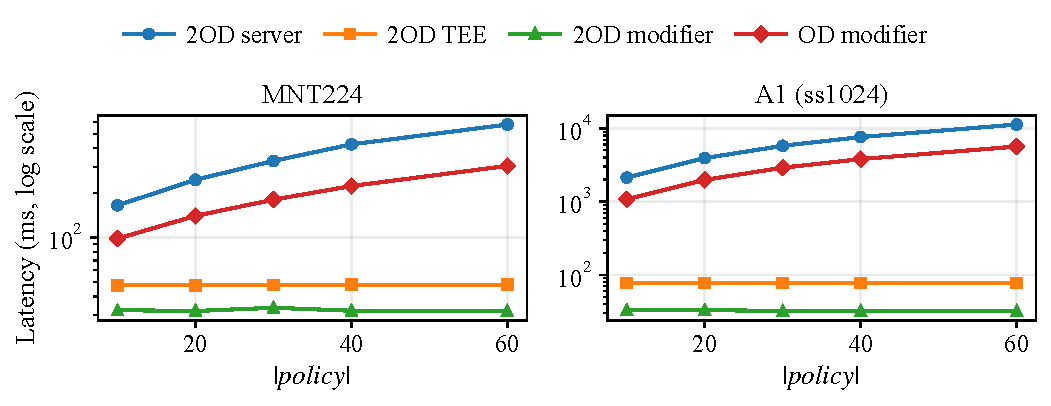
\includegraphics[width=0.84\textwidth]{../targeted_tables/figures/adaptation_latency.pdf}
\caption{Adaptation latency split on MNT224 and A1.}
\label{fig:targeted-adaptation}
\end{figure*}

\begin{table*}[t]
\centering
\caption{Adaptation latency across policy sizes (ms), $|\mathbb{S}|=60$.}
\scriptsize
\TableStyle
\resizebox{\textwidth}{!}{\begin{tabular}{c rr rr rr rr rr}
\toprule
\multirow{3}{*}{$|policy|$} & \multicolumn{6}{c}{\textbf{CHET-2OA + ABE-2OD}} & \multicolumn{4}{c}{\textbf{CHET-OA + ABE-OD}} \\
\cmidrule(lr){2-7}\cmidrule(lr){8-11}
 & \multicolumn{2}{c}{\textbf{Server}} & \multicolumn{2}{c}{\textbf{TEE}} & \multicolumn{2}{c}{\textbf{Modifier}} & \multicolumn{2}{c}{\textbf{TEE}} & \multicolumn{2}{c}{\textbf{Modifier}} \\
\cmidrule(lr){2-3}\cmidrule(lr){4-5}\cmidrule(lr){6-7}\cmidrule(lr){8-9}\cmidrule(lr){10-11}
 & \textbf{MNT} & \textbf{A1} & \textbf{MNT} & \textbf{A1} & \textbf{MNT} & \textbf{A1} & \textbf{MNT} & \textbf{A1} & \textbf{MNT} & \textbf{A1} \\
\midrule
10 & 164.9 & 2127.3 & 47.6 & 77.5 & 32.3 & 33.0 & 50.7 & 79.6 & 98.3 & 1071.1 \\
20 & 245.3 & 3915.3 & 47.6 & 77.5 & 31.9 & 33.0 & 51.8 & 80.6 & 140.0 & 1976.3 \\
30 & 329.2 & 5766.7 & 47.7 & 77.4 & 33.6 & 32.2 & 50.4 & 79.6 & 180.2 & 2899.0 \\
40 & 425.5 & 7588.3 & 48.0 & 77.2 & 32.0 & 32.3 & 50.6 & 80.2 & 222.6 & 3797.3 \\
60 & 579.1 & 11248.6 & 47.9 & 77.5 & 31.9 & 32.1 & 50.1 & 79.3 & 304.7 & 5636.2 \\
\bottomrule
\end{tabular}
}
\label{tab:targeted-adaptation}
\end{table*}

\subsection{Hash-check Benefit}
We also isolate the user-side benefit of the final hash-check trick. The strict legacy comparison now measures a full re-encryption-based finalize path rather than the earlier lightweight AES-only check.

\begin{figure*}[t]
\centering
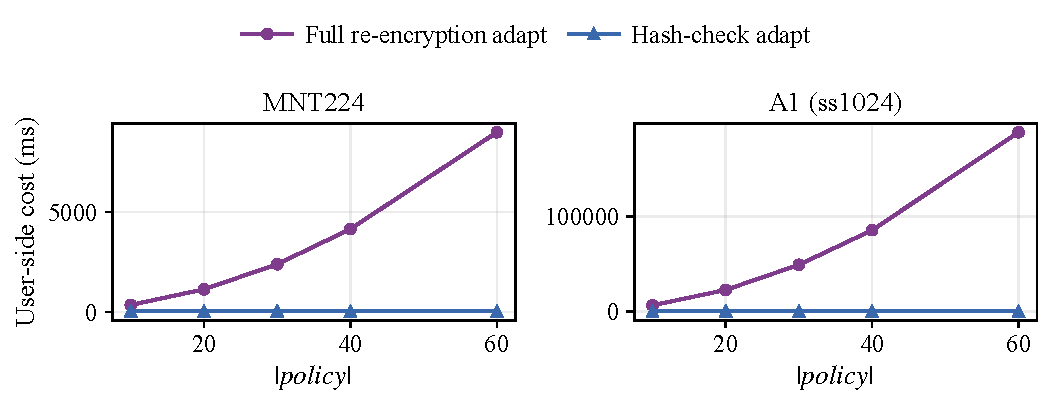
\includegraphics[width=0.84\textwidth]{../targeted_tables/figures/hashcheck_vs_reenc.pdf}
\caption{Full re-encryption finalization versus hash-check finalization.}
\label{fig:targeted-hashcheck}
\end{figure*}

\begin{table*}[t]
\centering
\caption{User-side finalization comparison (ms).}
\scriptsize
\TableStyle
\resizebox{\textwidth}{!}{\begin{tabular}{c rr rr}
\toprule
\multirow{2}{*}{$|policy|$} & \multicolumn{2}{c}{\textbf{Full Re-encryption Adapt}} & \multicolumn{2}{c}{\textbf{Hash-check Adapt}} \\
\cmidrule(lr){2-3}\cmidrule(lr){4-5}
 & \textbf{MNT} & \textbf{A1} & \textbf{MNT} & \textbf{A1} \\
\midrule
10 & 355.1 & 6427.3 & 32.3 & 33.0 \\
20 & 1136.5 & 22702.4 & 31.9 & 33.0 \\
30 & 2389.6 & 49164.1 & 33.6 & 32.2 \\
40 & 4148.7 & 85640.4 & 32.0 & 32.3 \\
60 & 8977.5 & 188760.0 & 31.9 & 32.1 \\
\bottomrule
\end{tabular}
}
\label{tab:targeted-hashcheck}
\end{table*}

\subsection{Revocation Comparison}
For revocation, we compare only with server-assisted revocation designs, namely EHR-RPCH and TAR-PCH, together with our TEE-RPCH state-signing and TEE-check path.

\begin{figure*}[t]
\centering

\includegraphics[width=0.84\textwidth]{../targeted_tables/figures/revocation_comparison.pdf}
\caption{Revocation cost for one modifier on MNT224 and A1.}
\label{fig:targeted-revocation}
\end{figure*}

\begin{table*}[t]
\centering
\caption{Revocation cost for one revoked modifier (ms).}
\scriptsize
\TableStyleTight
\resizebox{\textwidth}{!}{\input{../targeted_tables/tables/table4_revocation.tex}}
\label{tab:targeted-revocation}
\end{table*}

\FloatBarrier

\section{Conclusion}
The MNT224 preview confirms that the current figure and table assets can be embedded into the target paper format. The full report still needs the corresponding A1 measurements before the final experimental section can be completed.

% \input{sections/backmatter}

\FloatBarrier
\bibliographystyle{ACM-Reference-Format}
\bibliography{reference}

\FloatBarrier
\appendix %% CCS: DO NOT REMOVE

\section{Open Science} %% CCS: DO NOT REMOVE

The artifacts needed to evaluate the experimental claims of this paper include the TEE-RPCH implementation, benchmark scripts, plotting scripts, configuration files, and raw timing logs. These artifacts will be provided to the program committee through an anonymous artifact package for double-blind review. No external user data or proprietary datasets are required to reproduce the reported cryptographic and systems measurements.

\section{Ethical Considerations}

This work studies a cryptographic primitive and its TEE-assisted revocation mechanism. It does not involve human subjects, user data, or real-world vulnerability disclosure. The main security risk is misuse of redactable mechanisms to perform unauthorized history modification; our construction is designed to restrict rewriting to authorized modifiers and to support revocation of such privileges.

\section{Additional Material}
No additional appendix material is included in this preview build.


\end{document}
